\documentclass{article}

\usepackage[%
    left=0.5in,%
    right=0.5in,%
    top=0.5in,%
    bottom=0.5in,%
]{geometry}%
\usepackage{minitoc}
\usepackage{multicol}
\usepackage{graphicx}
\usepackage{fixltx2e}
\usepackage{listings}
\usepackage{color}
\usepackage{hyperref}
    \hypersetup{ colorlinks = true, linkcolor = blue }
\usepackage{blindtext}
\definecolor{lightgray}{gray}{0.9}
\graphicspath{ {./} }

\newcommand{\inlinecode}[2]{\colorbox{lightgray}{\lstinline
[language=#1]$#2$}}
\newcommand{\worddef}[1]{\hyperref[sec:reference]{\textit{#1}}}

\begin{document}

\tableofcontents

\newpage

\section{Designing intelligent agents}
\begin{itemize}
  \item an \worddef{agent} operates in a task environment:
  \begin{itemize}
    \item \textit{task}: the goal(s) the agent is trying to achieve
    \item \textit{environment}: that part of the real world or a computational system ‘inhabited’ by the agent 
  \end{itemize}
  \item agent obtains information about the environment in the form of percepts 
  \item agent changes the environment by performing actions to achieve its goals
\end{itemize}

\section{From agent functions to agent programs}

\begin{itemize}
  \item the \textbf{behaviour} of an agent is described by an \worddef{agent function} (action selection function) which maps a goal and sequence of percepts to an action (and possibly results)
  \item agent programming is conventionally conceived as the problem of
synthesising an agent function
  \item  Difficult to design, because of unknown environments.
\end{itemize}

\section{Agent architectures}

\begin{itemize}
  \item one way of making the agent programming problem more tractable is make use of the notion of an agent architecture 
  \item the notion of an “agent architecture” is ubiquitous in the agent literature but is not well analysed 
  \item often discussed in the context of an agent programming language or platform 
  \item architecture is a blueprint for software agents and intelligent control systems, depicting the arrangement of components
\end{itemize}

\subsection{Russell and Norvig view of an agent}

\begin{multicols}{2}

\begin{itemize}
  \item \textbf{program}: implements the agent function mapping from goals and percepts to actions (and results) 
  \item \textbf{state}: includes all the internal representations on which the agent program operates 
  \item \textbf{architecture}: computing device with sensors and actuators that runs the agent program
\end{itemize}

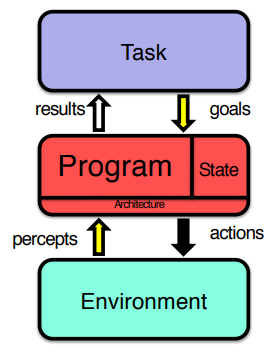
\includegraphics[scale=0.5]{russel_norvig_agent.png}

\end{multicols}

\subsection{Architecture as a virutal machine}

\begin{itemize}
  \item the architecture defines a (real or virtual) machine which runs the agent program 
  \item defines the atomic operations of the agent program and implicitly determines the components of the agent 
  \item determines which operations happen automatically, without the agent program having to do anything 
  \item e.g., the interaction between memory, learning and reasoning   
  \item an architecture constrains kinds of agent programs we can write (easily)
\end{itemize}

\pagebreak

\subsection{Architectural view of an agent} 

\begin{multicols}{2}

\begin{itemize}
  \item \textbf{program}: a function mapping from goals and percepts to actions (and results) expressed in terms of virtual machine operations 
  \item \textbf{state}: the virtual machine representations on which the agent program operates 
  \item \textbf{architecture}: a virtual machine that runs the agent program and updates the agent state
\end{itemize}

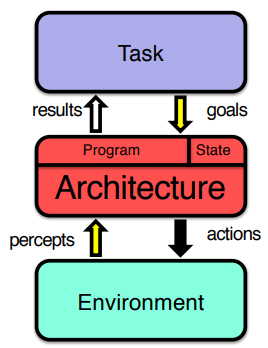
\includegraphics[scale=0.5]{architectural_agent_view.png}

\end{multicols}

\subsection{Hierarchies of virtual machines}

\begin{flushleft}
In many agents we have a whole hierarchy of virtual machines, used without qualification, ‘agent architecture’ means the most abstract architecture or the highest level virtual machine
\end{flushleft}

\section{Cognitive architecture}

\begin{itemize}
  \item agent architecture is also related to the notion of a cognitive architecture as used in artificial intelligence and cognitive science 
  \item a \textit{cognitive architecture} is an integrated system capable of supporting intelligence 
  \item often used to denote models of \textbf{human reasoning}, e.g., ACT-R, SOAR 
  \item in other cases no claims about psychological plausibility are made 
  \item in this latter sense, cognitive architecture is more or less synonymous with agent architecture as used here
\end{itemize}

\subsection{Properties of the architecture}

\begin{itemize}
  \item an agent architecture can be seen as defining a class of agent programs 
  \item just as individual agent programs have properties that make them more or less successful in a given task environment 
  \item architectures (classes of programs) have higher-level properties that determine their suitability for a task environment 
  \item choosing an appropriate architecture can make it much easier to develop an agent program for a particular task environment
  \item to program an agent which is successful in a given task environment, we must choose an architecture which is \textbf{appropriate} for that task environment
\end{itemize}

\pagebreak

\section{Task environments and architectures}
\begin{flushleft}
To choose an architecture which is appropriate for a given task environment we must be able to characterise both task environments and architectures
\end{flushleft}

\subsection{The task environment defines the problem}

\begin{multicols}{2}
\begin{itemize}
  \item we can sometimes \textbf{manipulate} the task and/or environment to make things easier 
  \item e.g., increasing the contrast of objects to make things easier for a robot’s cameras 
  \item however the task environment is usually given
\end{itemize}

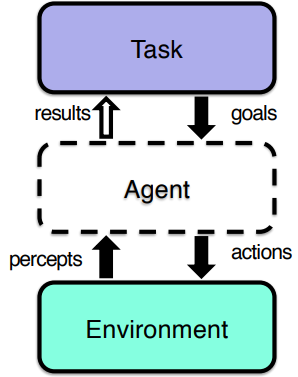
\includegraphics[scale=0.5]{task_environment.png}

\end{multicols}

\subsection{Specifying task and environment}

\begin{multicols}{2}
\begin{itemize}
  \item the task specifies the \textbf{goals} the agent must achieve (and any results required) 
  \item the agent (architecture) and environment \textbf{jointly determine}:
  \begin{itemize}
    \item the information the agent can obtain (percepts)
    \item the actions the agent can perform 
  \end{itemize}
  \item decomposition into task and environment is not always obvious
\end{itemize}

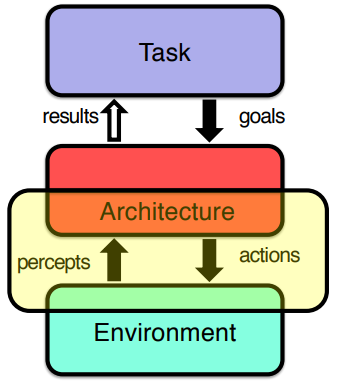
\includegraphics[scale=0.5]{specifying_task.png}

\end{multicols}

\subsubsection{Specifying the task}
\begin{itemize}
  \item some tasks may come from the \textbf{agent itself} (autonomy) 
  \item an agent may generate its own (top-level) \textbf{goals} 
  \item e.g., may generate a goal to keep its battery charged 
  \item or it may make use of its own results, e.g., in learning
\end{itemize}

\subsubsection{Specifying the environment}
\begin{itemize}
  \item similarly, an agent may be \textbf{part of its own environment}
  \item e.g., if it has sensors monitoring its battery level 
  \item agent may also form part of the environment of other agents 
  \item e.g., in a multi-agent system
\end{itemize}

\section{Task environment classification}
\begin{itemize}
  \item Will classify the agent’s \textbf{task environment} based on:
  \begin{itemize}
    \item \textbf{task}: properties of the goals that must be achieved
    \item \textbf{environment}: \textbf{properties} of the percepts and \textbf{actions} possible in the environment 
  \end{itemize}
  \item the following properties are illustrative only—for particular types of task environments other properties may be more useful
  \item we assume that it is possible to view the agent as an \textit{intentional system}, i.e., that we can \textbf{ascribe a set of goals} to it which characterise its behaviour
\end{itemize}

\section{Properties of the task}

\begin{itemize}
  \item \textbf{type of goal}: a goal to achieve a particular state in the environment is termed an \textbf{achievement goal}; a goal to maintain or preserve a state in the environment is termed a \textbf{maintenance goal} 
  \item \textbf{number of goals}: if the agent must achieve multiple goals in parallel, we say the agent has multiple goals, otherwise it has a single goal 
  \item \textbf{commitment to goals}: if a goal is only abandoned when it is achieved we say the agent is \textbf{strongly committed} to its goal(s); otherwise it is only \textbf{weakly committed }
  \item \textbf{utilities of goals}: if the reward for achieving each goal is the same, we say the agent’s goals have equal utility; otherwise its goals have differing utilities 
  \item \textbf{constraints on how goals are achieved}: e.g., deadlines, resource bounds
\end{itemize}

\section{Properties of the environment (percepts)}

\begin{itemize}
  \item \textbf{discrete / continuous}: if there are a limited number of distinct, clearly defined, states of the environment, the environment is discrete; otherwise it is continuous.
  \begin{itemize}
    \item Analysing email is a continuous environment, where as a game of chess or checkers where there are a set number of moves is descrete.
  \end{itemize}
  \item \textbf{observable / partially observable}: if it is possible to determine the complete state of the environment at each time point from the percepts it is observable; otherwise it is only partially observable.
  \begin{itemize}
    \item Checker board is a complete environment because the agent has complete knowledge of the board, where as a game of cards is partially observable as oponent cards can't be seen
  \end{itemize}
  \item \textbf{static / dynamics}: if the environment only changes as a result of the agent’s actions, it is static; otherwise it is dynamic
  \begin{itemize}
    \item Empty office with no moving objects is a static environment, where as physical world would be dynamic
  \end{itemize}
  \item \textbf{deterministic / nondeterministic}: if the future state of the environment can be predicted in principle given the current state and the set of actions which can be performed, it is deterministic; otherwise it is nondeterministic 
  \begin{itemize}
    \item Tic Tac Toe game is deterministic, where as a robot on mars is nondeterministic
  \end{itemize}
  \item \textbf{single agent / multiple agents}: the environment may contain other agents which may be of the same kind as the agent, or of different kinds
  \begin{itemize}
    \item A conveyor belt would have multiple agents, where as sewing machine robot would be a single agent environment.
  \end{itemize}
\end{itemize}

\section{Properties of the environment (actions)}

\begin{itemize}
  \item \textbf{fallibility of actions}: an action is infallible if it is guaranteed to produce its intended effects when executed in an environment which satisfies the preconditions of the action; otherwise it is fallible 
  \item \textbf{utility of actions}: the utility of an action is the utility of the state which results from the action–the action with maximum utility is correct 
  \item \textbf{costs of actions}: the resource cost of performing the action– an action is optimal if it is correct and there is no other correct action with lower cost 
  \item \textbf{communicating actions}: an agent can be said to communicate with other agents in a meaningful way if it interacts with them via some kind of agent communication language
\end{itemize}

\section{Architecture}

\subsection{Tasks and architecture}

\begin{itemize}
  \item if the agent has at least one \textit{maintenance goal}, then the agent’s ‘lifetime’ is potentially \textbf{unbounded} 
  \item if the agent must pursue \textit{multiple goals} in parallel, it needs some way of choosing which goal it should be working on at the moment 
  \item if the agent is only \textit{weakly committed} to its goals, it needs to be able to be able to decide when it should give up trying to pursue a goal 
  \item if the \textit{utilities} of the agent’s goals differ, then its commitment to a goal may change and/or the agent needs to be able to determine which goal it should be pursuing at any given time
\end{itemize}

\subsection{Percepts and architecture}

\begin{itemize}
  \item discrete environments are usually \textbf{easier to represent} than continuous ones 
  \item if the environment is only partially observable, \textit{internal state} is required to keep track of the current state of the world 
  \item if the environment is dynamic, then \textit{the time it takes the agent to choose} which action to perform becomes important 
  \item if the environment is nondeterministic, then any representation or reasoning capabilities will probably require a \textbf{notion of uncertainty}
\end{itemize}

\subsection{Actions and architecture}

\begin{itemize}
  \item if actions are infallible, the agent \textbf{does not need to monitor} the environment to tell whether an action has succeeded 
  \item if actions have varying costs and/or utilities and the agent wants to \textbf{minimise cost or maximise utility}, it needs to be able to choose between alternative courses of action 
  \item if the agent can communicate with other agents, it must \textbf{decide} what to communicate and when, and what to do with information it receives from other agents
\end{itemize}

\pagebreak
\section*{Reference section} \label{sec:reference}
\begin{description}
	\item[agent function] \hfill \\ The agent function is a mathematical function that maps a sequence of perceptions into action
	\item[agent] \hfill \\ In artificial intelligence, an intelligent agent (IA) is an autonomous \textbf{entity}, which observes through sensors and acts upon an environment using actuators and directs its activity towards achieving goal
\end{description}
\end{document}
